\section{Model Training}

\subsection{SRCNN}
\begin{frame}{SRCNN}{Super Resolution CNN \href{https://github.com/yjn870/SRCNN-pytorch}{GitHub Link}}
    
    \begin{figure}
        \centering
        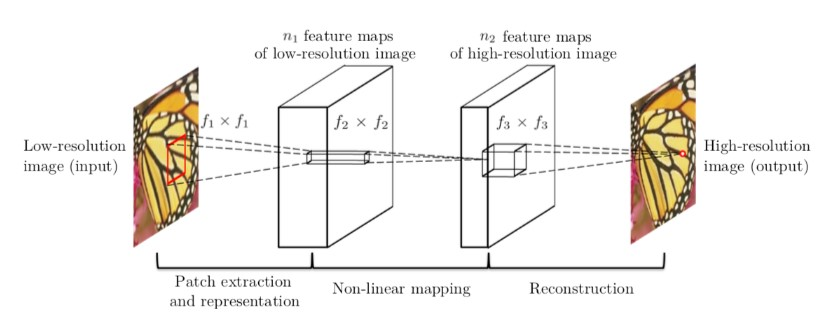
\includegraphics[height=3cm]{pic/pic0101.jpg}
        \caption{SRCNN}
        \label{fig:0101}
    \end{figure}

    训练前需要使用h5py库进行数据库制作提高IO效率

    在此步骤一直提示内存不足
    
    猜想图片分辨率较高, 因此占用内存较大.
\end{frame}

\begin{frame}{SRCNN Result}
    \small 直接使用预训练模型结果
    \begin{figure}[!htbp]
        \centering
        \subfloat[input]{\label{fig:0201a}
        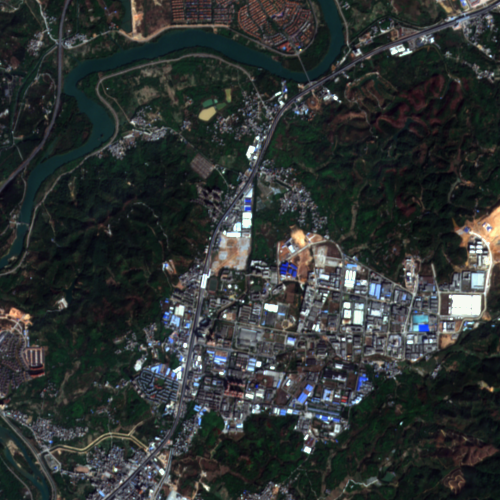
\includegraphics[height=4cm]{pic/pic0102a.png}}
        \quad
        \subfloat[output]{\label{fig:0201b}
        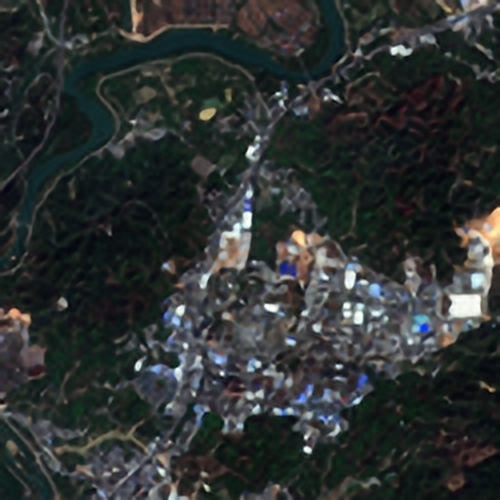
\includegraphics[height=4cm]{pic/pic0102b.png}}
        \caption{SRCNN预训练模型结果}
        \label{fig:0102}
    \end{figure}
    
\end{frame}

\subsection{EDSR}
\begin{frame}{EDSR}{Enhanced Deep Residual Networks \href{https://github.com/sanghyun-son/EDSR-PyTorch}{GitHub Link}}
    \begin{figure}
        \centering
        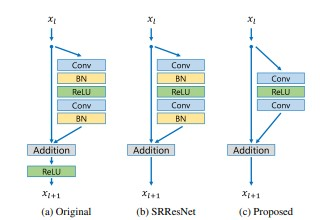
\includegraphics[height=3cm]{pic/pic0103.jpg}
        \caption{EDSR Residual Block}
        \label{fig:0103}
    \end{figure}

    尽管代码仓库有很多Star, 但其说明文档含糊不清. 

    训练报错训练集位置问题, 调试中

    使用预训练模型测试占用显存过大

    可用的命令和脚本都是在issue中找到

\end{frame}

\begin{frame}{EDSR Result} 
    \small
    \begin{figure}[!htbp]
        \centering
        \subfloat[input]{\label{fig:0104a}
        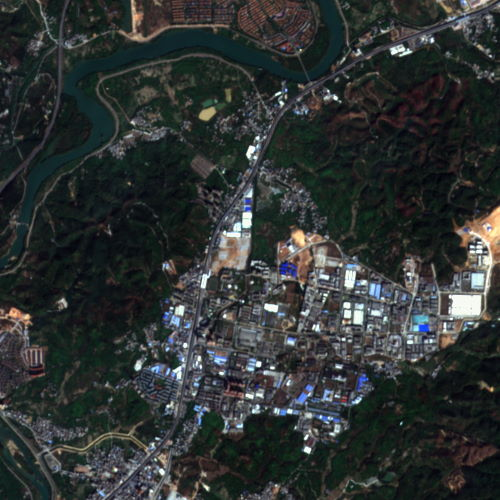
\includegraphics[height=4cm]{pic/pic0104a.jpg}}
        \quad
        \subfloat[output]{\label{fig:0104b}
        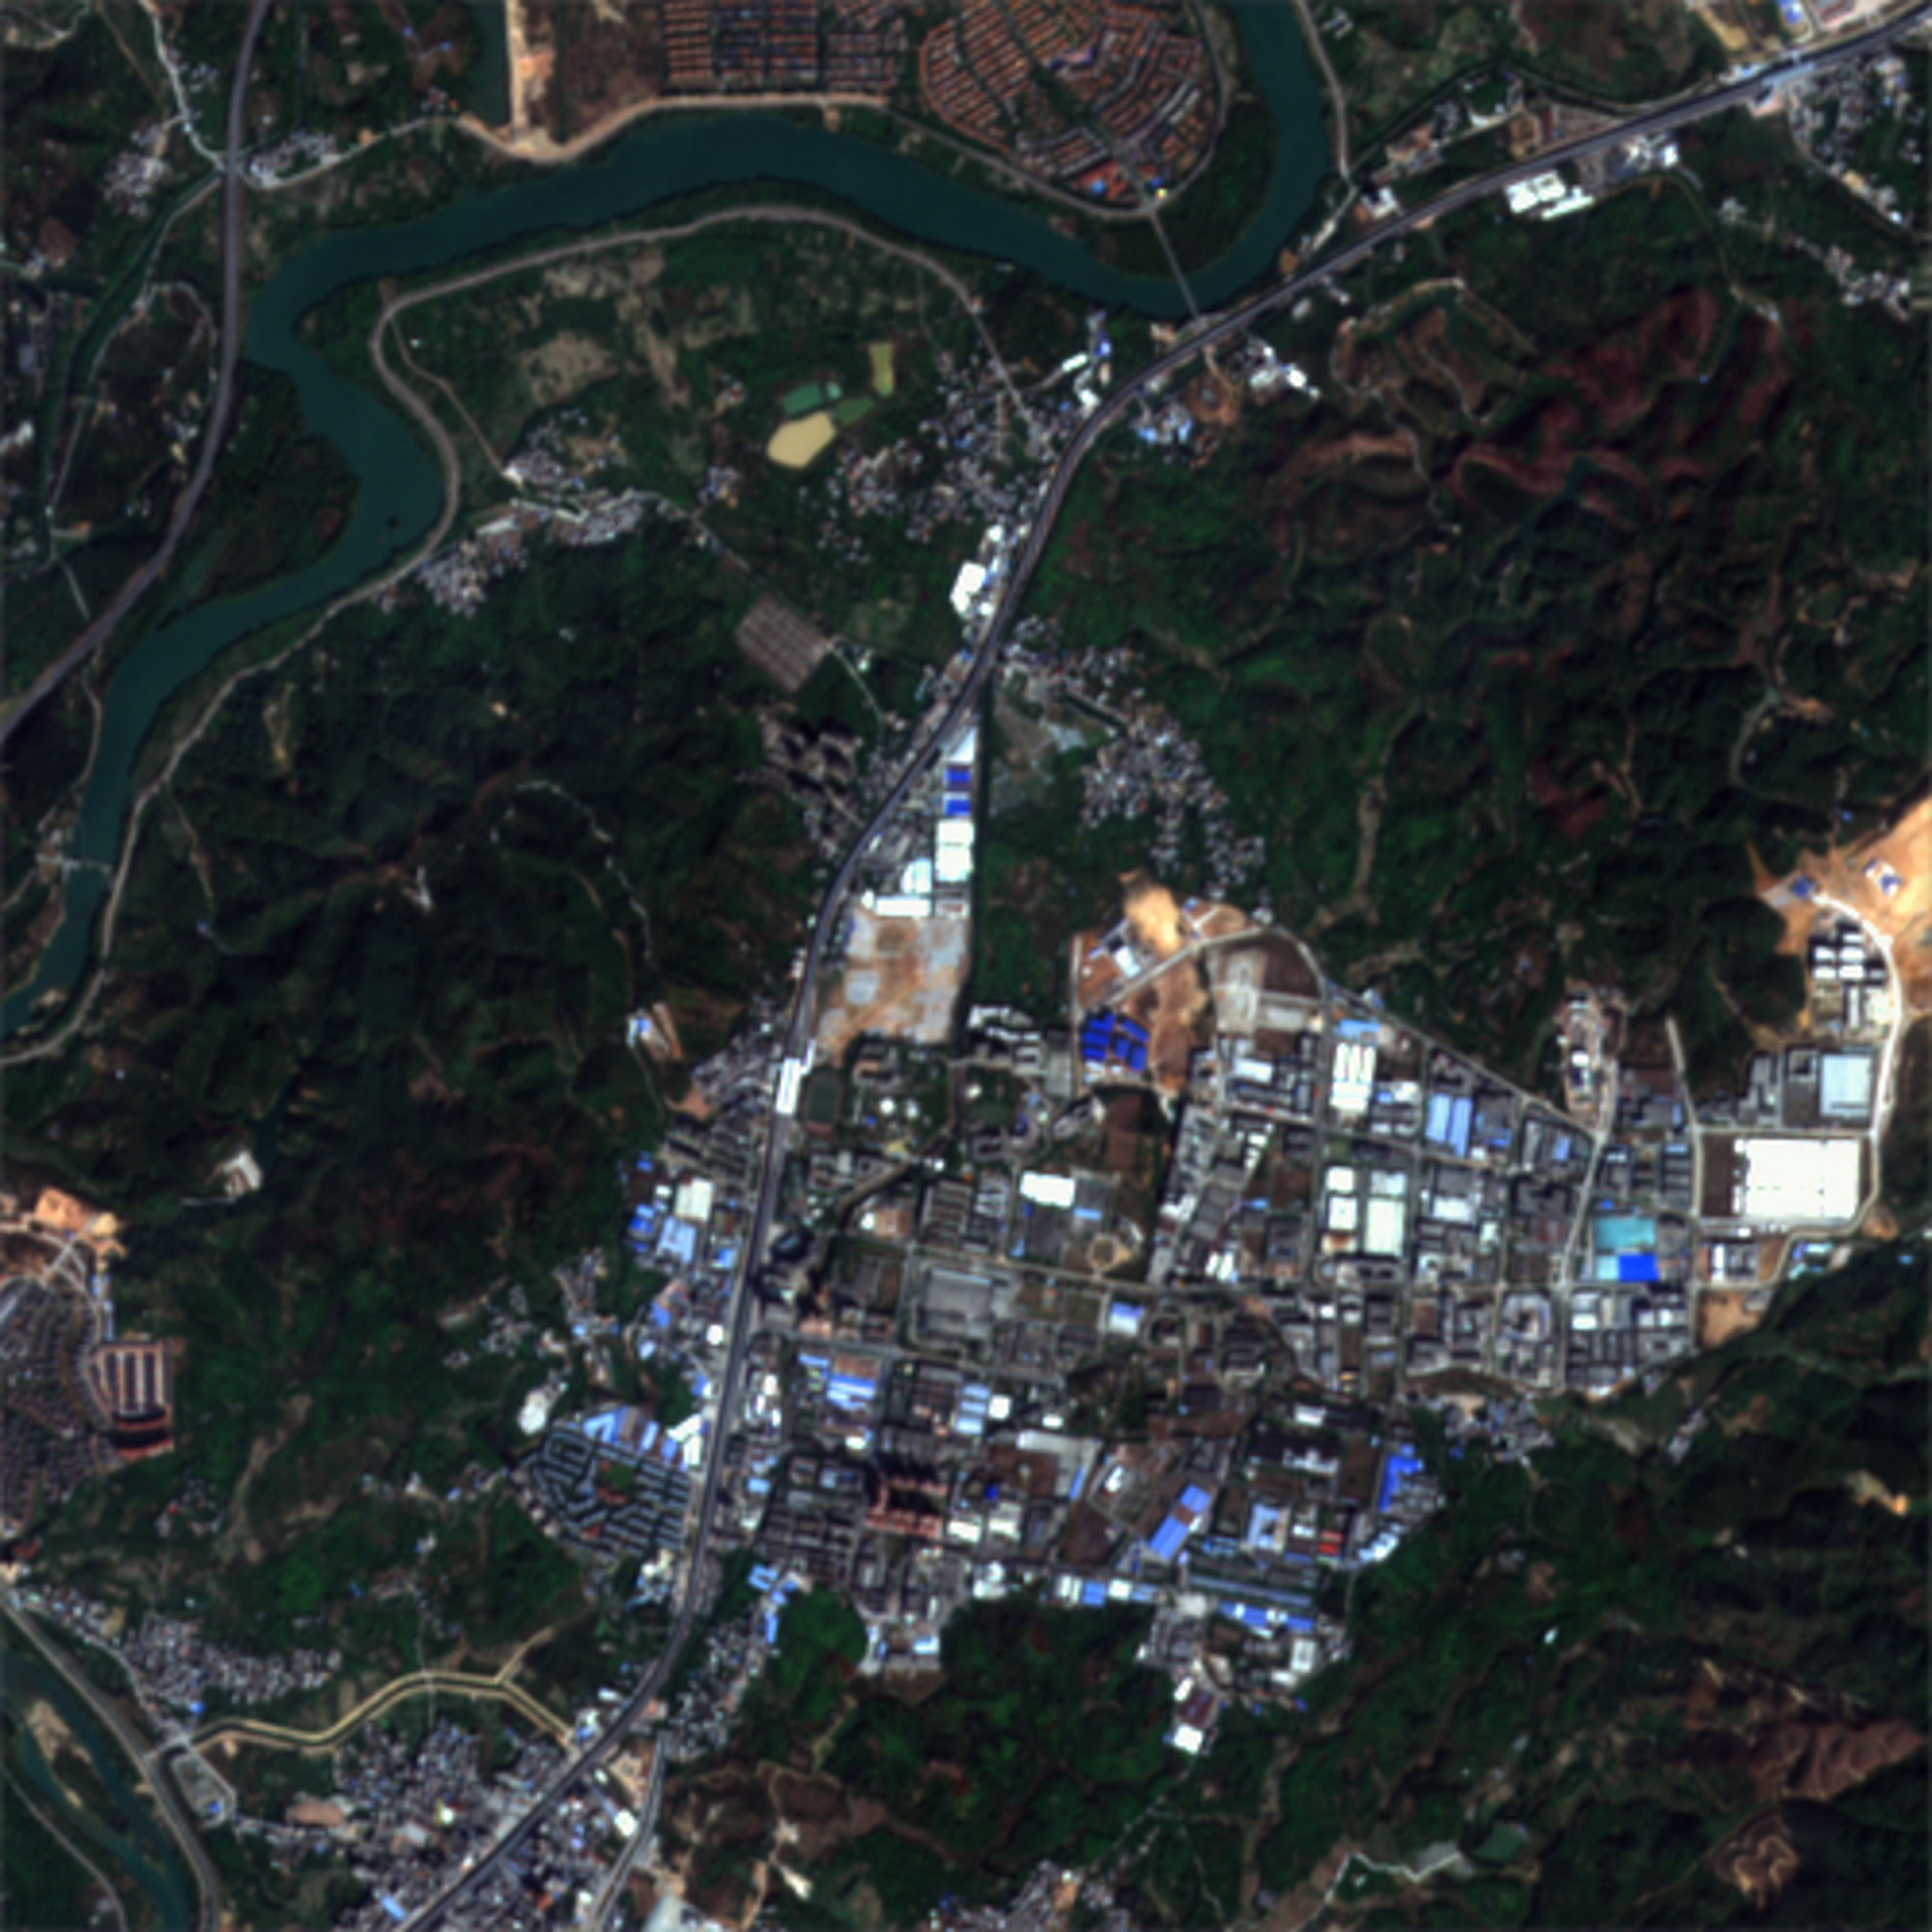
\includegraphics[height=4cm]{pic/pic0104b.jpg}}
        \caption{EDSR预训练模型结果}
        \label{fig:0104}
    \end{figure}
\end{frame}

\begin{frame}{EDSR Result}
    \small
    \begin{figure}[!htbp]
        \centering
        \subfloat[input]{\label{fig:0105a}
        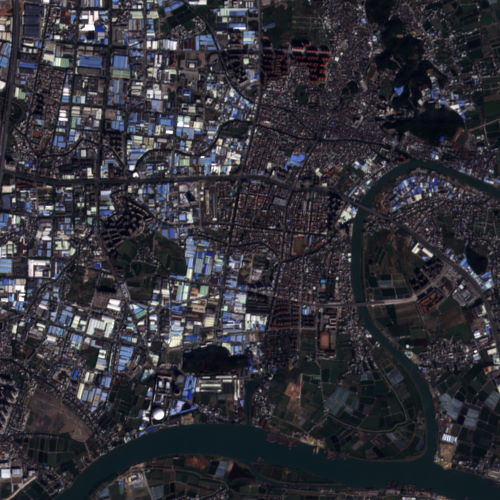
\includegraphics[height=4cm]{pic/pic0105a.jpg}}
        \quad
        \subfloat[output]{\label{fig:0105b}
        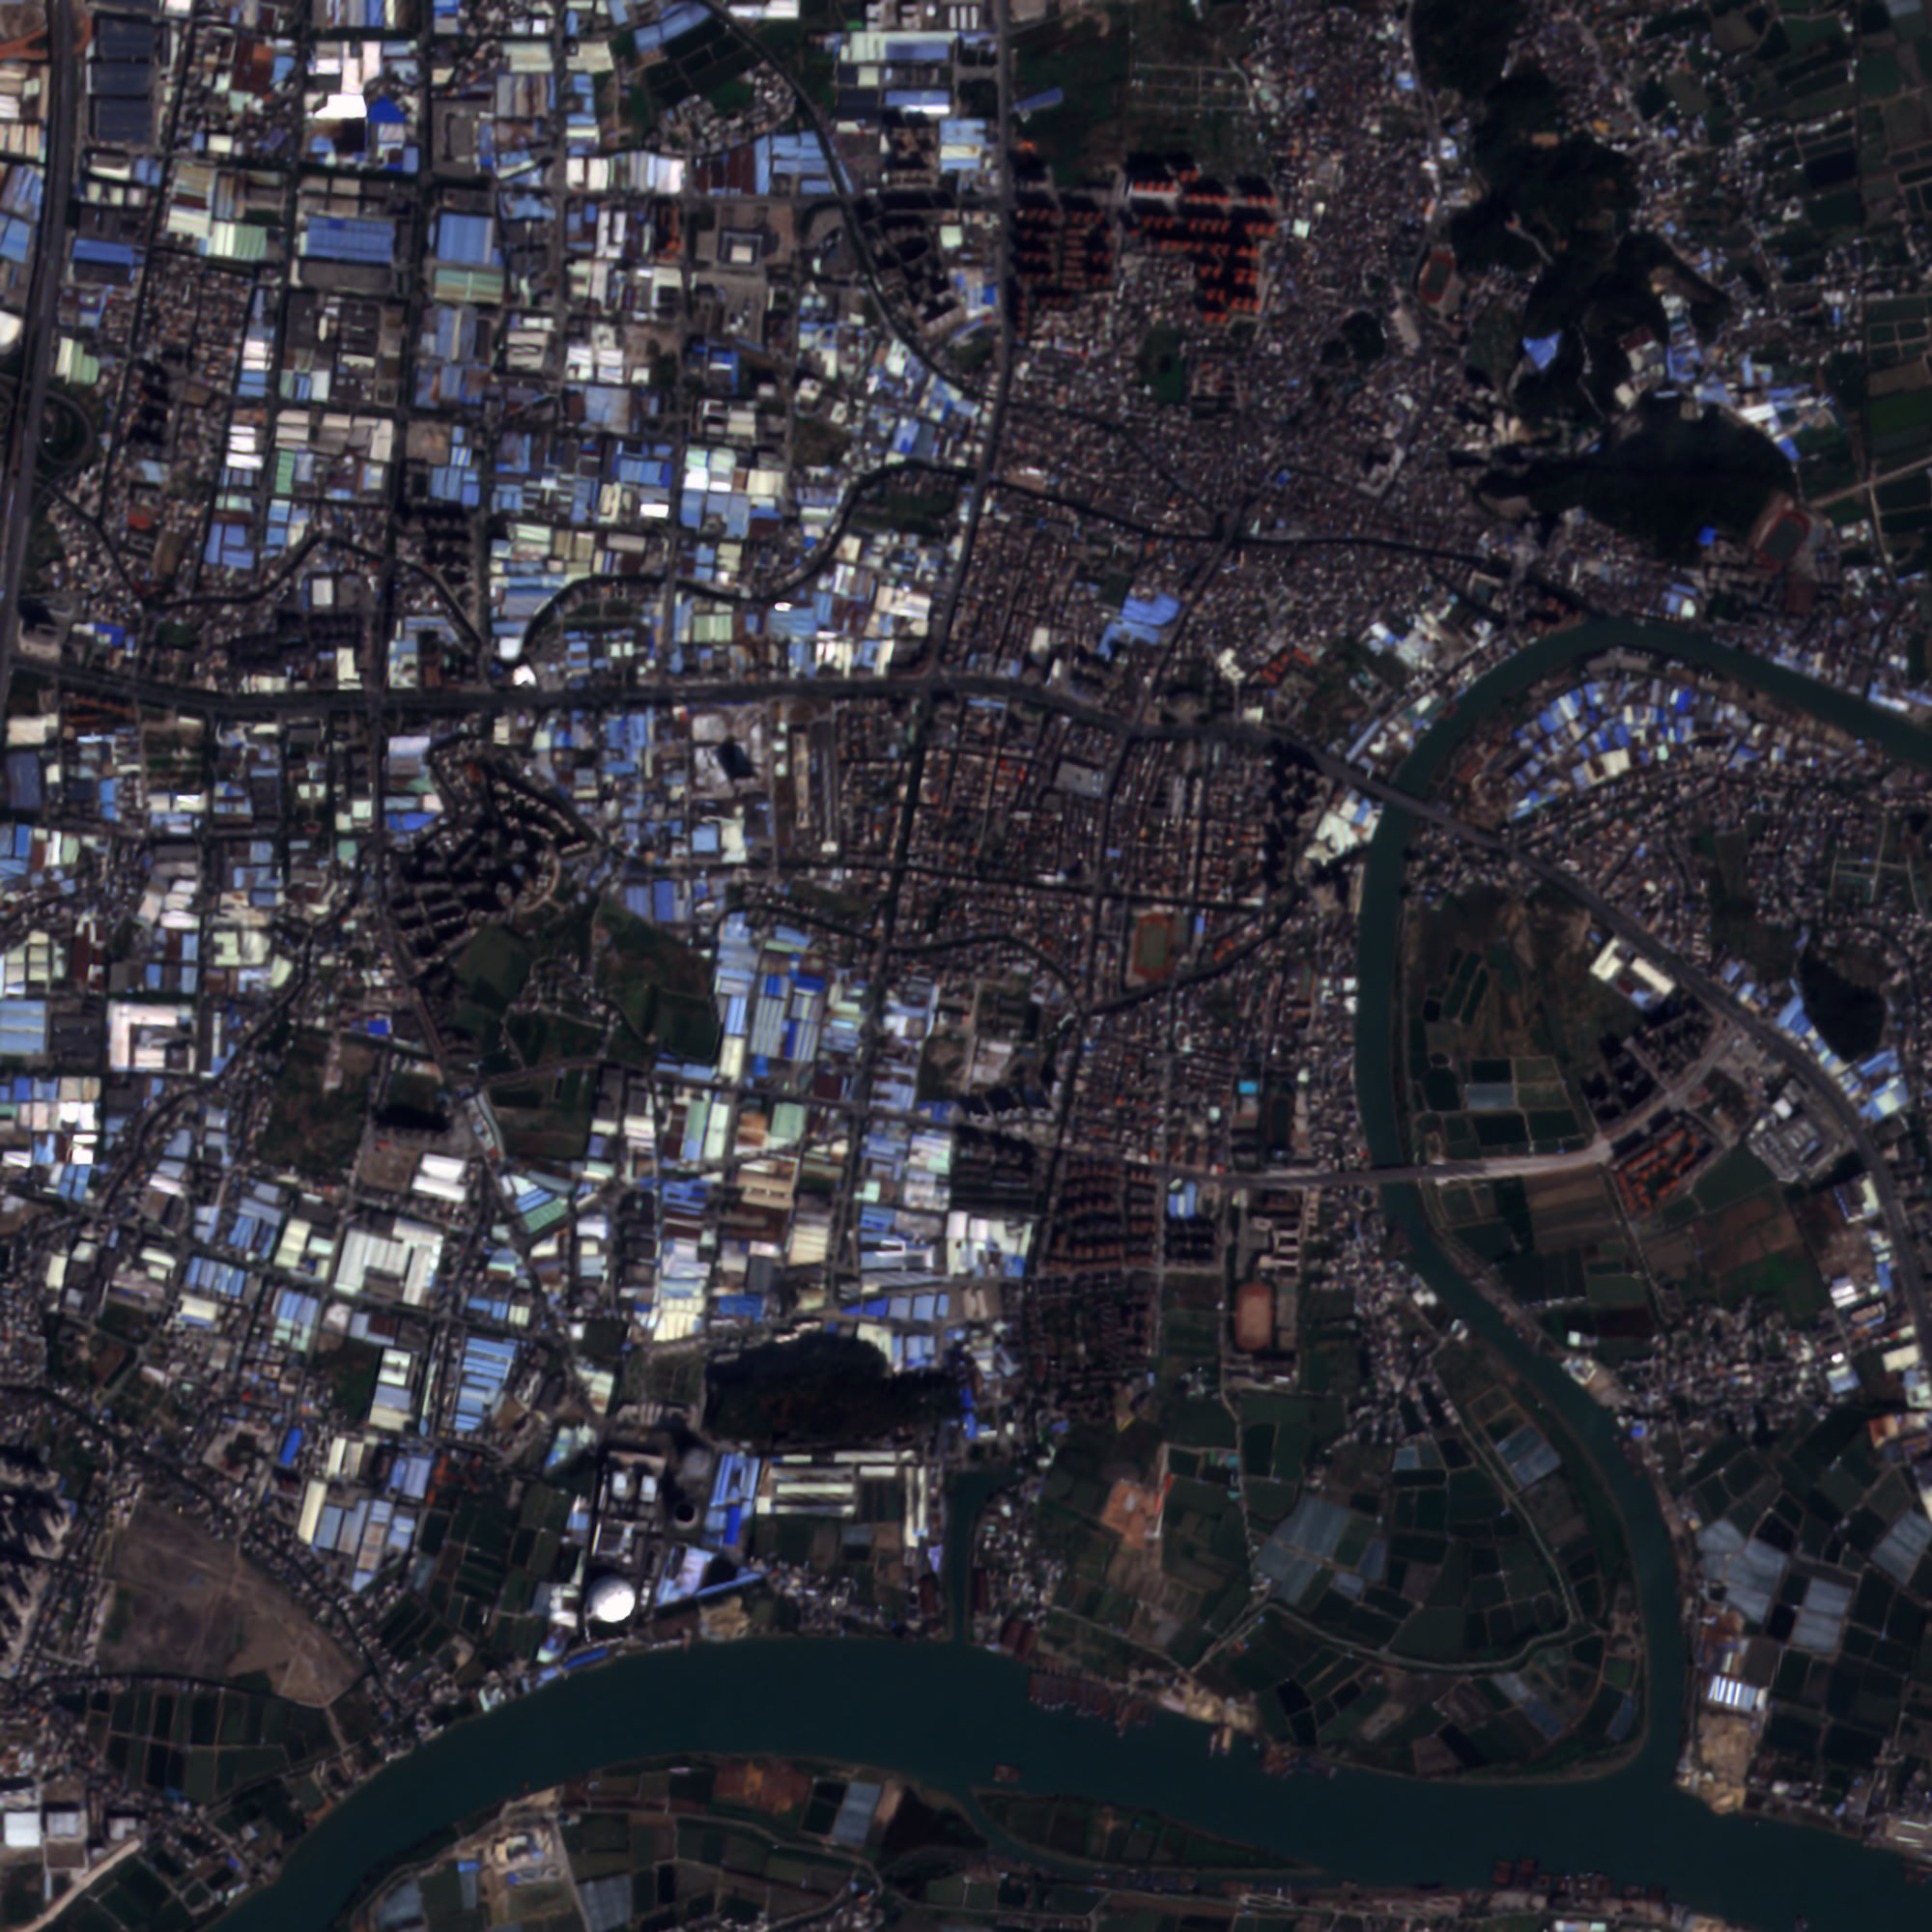
\includegraphics[height=4cm]{pic/pic0105b.jpg}}
        \caption{EDSR预训练模型结果}
        \label{fig:0105}
    \end{figure}
\end{frame}

\begin{frame}{EDSR Result}
    \small
    \begin{figure}[!htbp]
        \centering
        \subfloat[input]{\label{fig:0106a}
        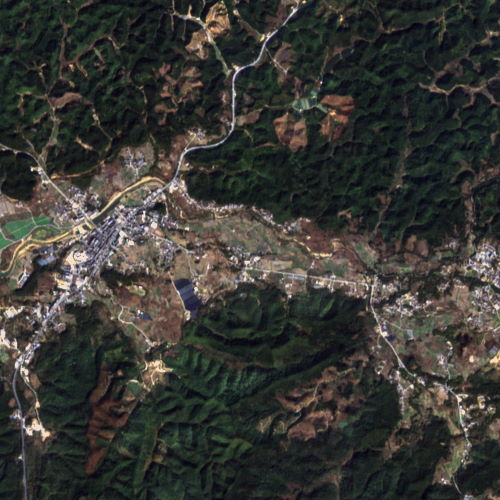
\includegraphics[height=4cm]{pic/pic0106a.jpg}}
        \quad
        \subfloat[output]{\label{fig:0106b}
        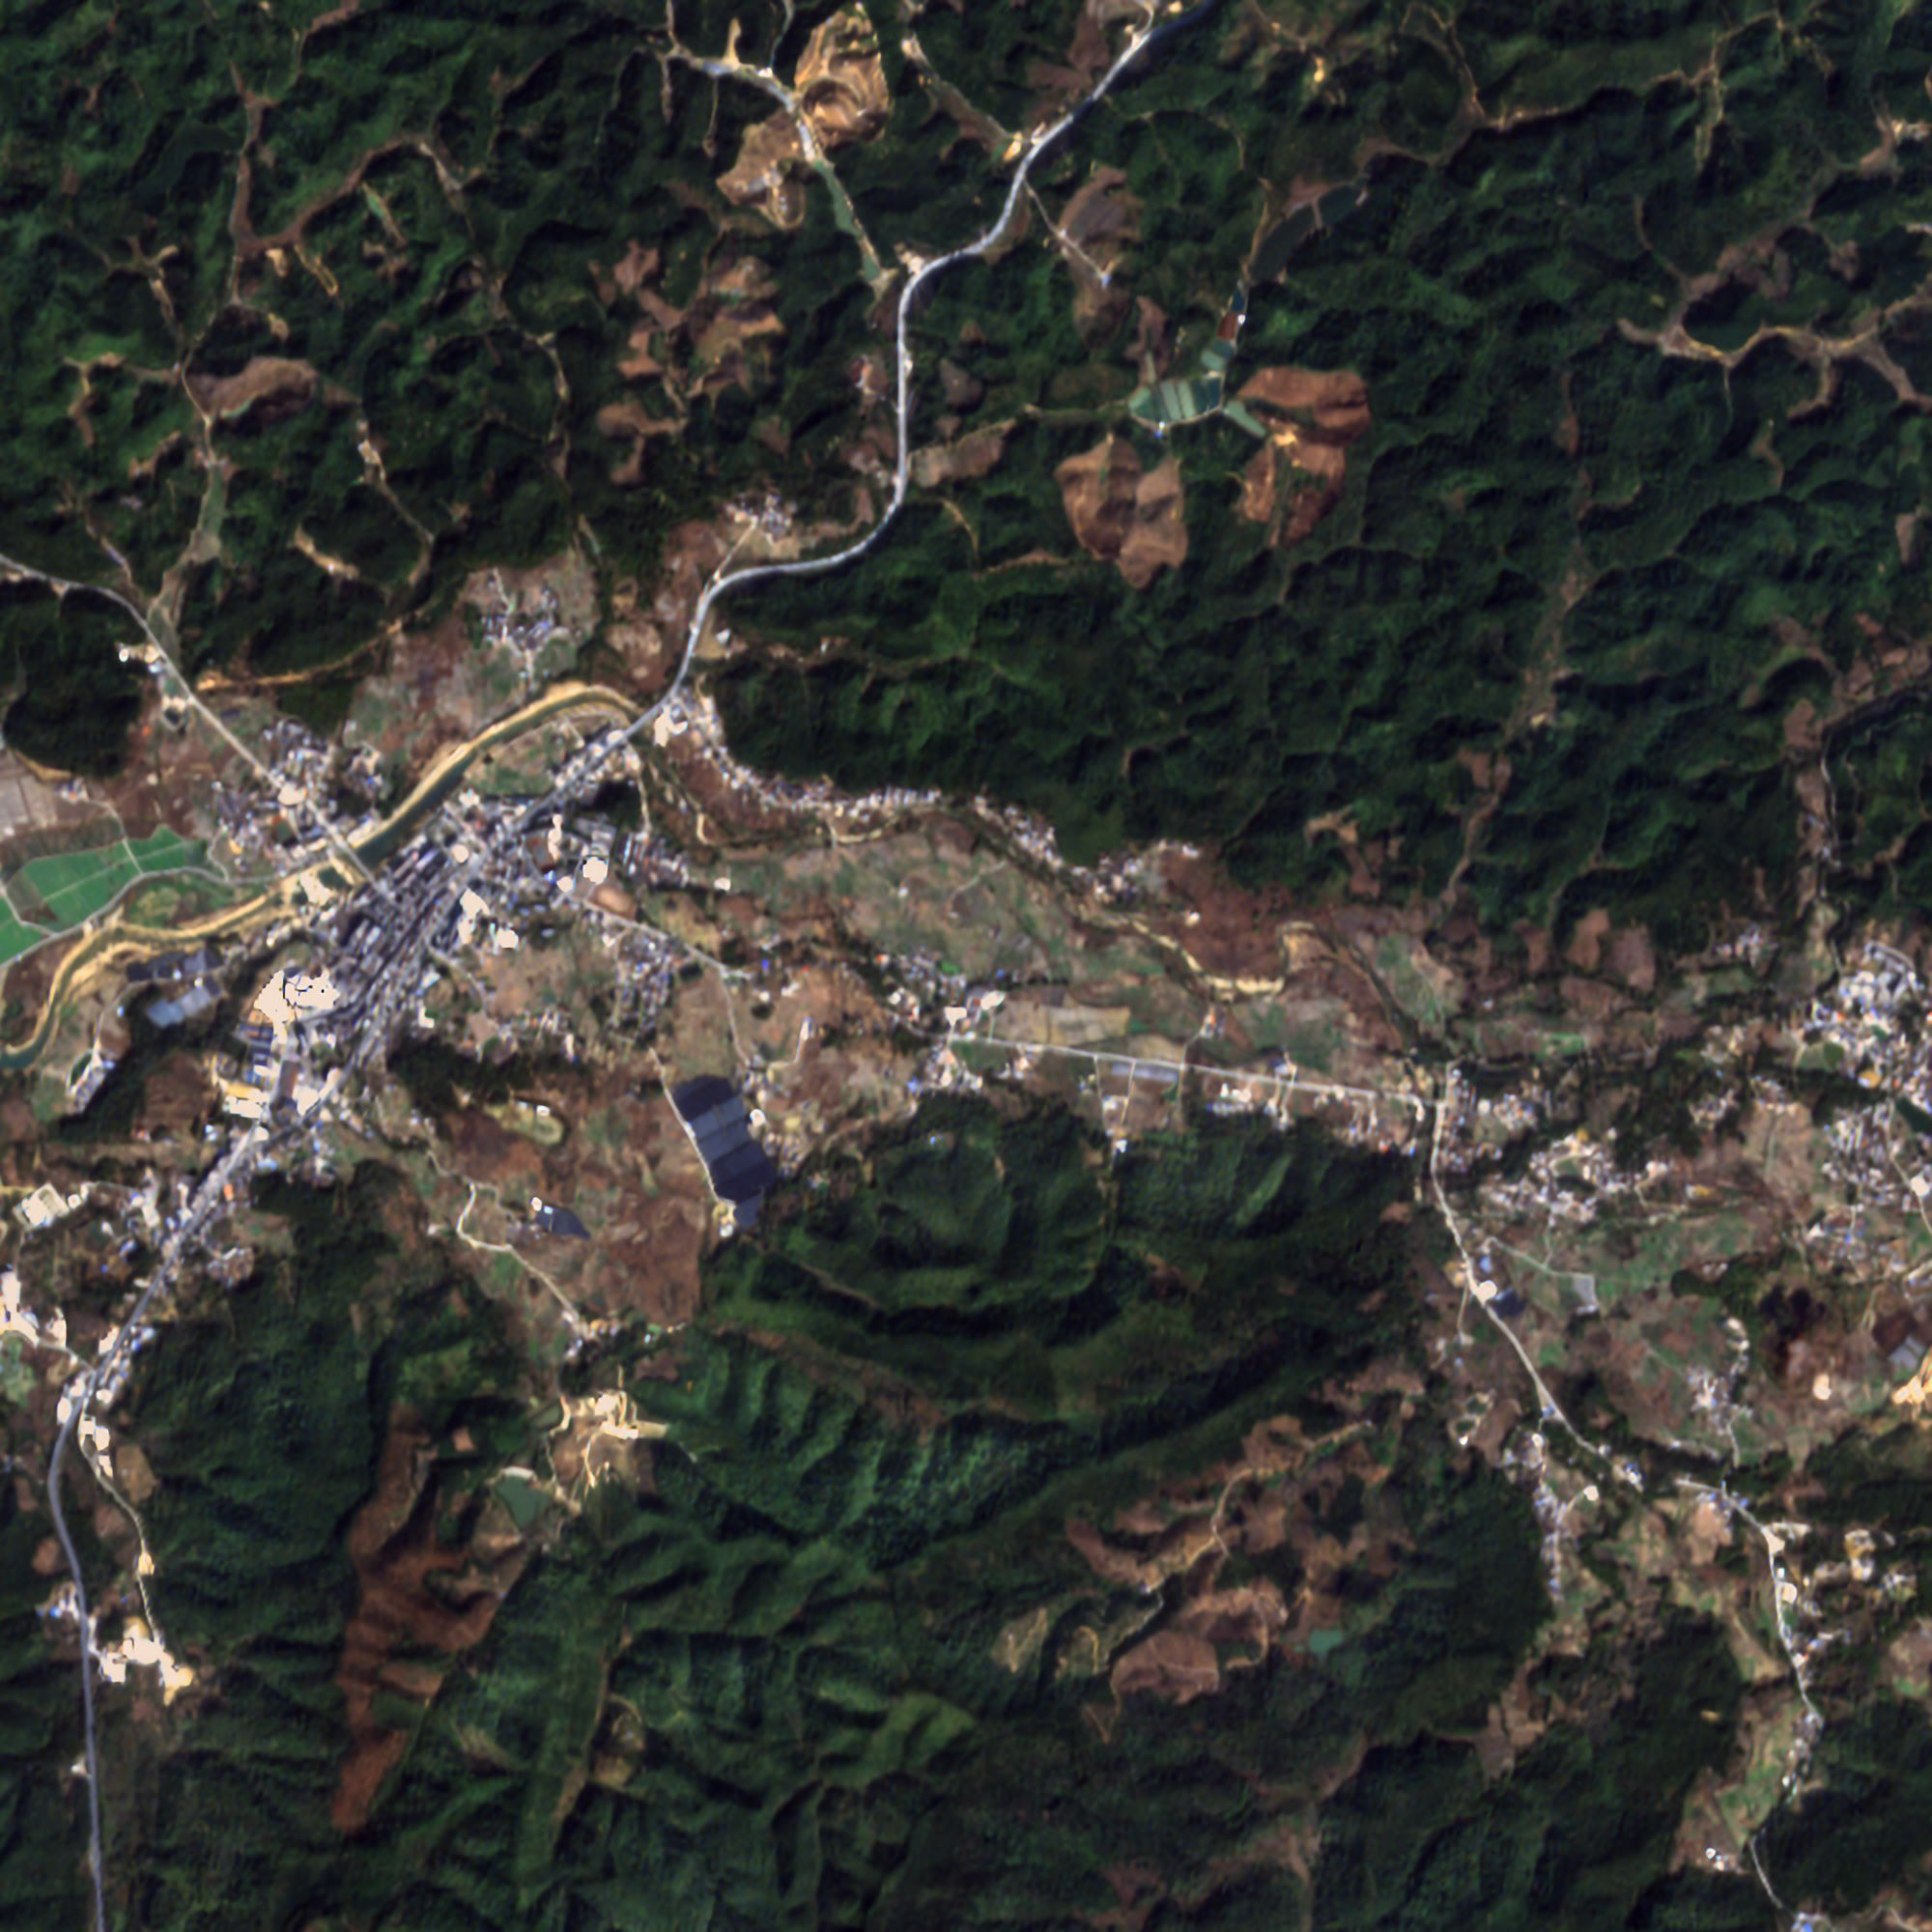
\includegraphics[height=4cm]{pic/pic0106b.jpg}}
        \caption{EDSR预训练模型结果}
        \label{fig:0106}
    \end{figure}
\end{frame}

\subsection{real-ESRGAN}
\begin{frame}{real-ESRGAN}{real Enhanced Super Resolution GAN \href{https://github.com/xinntao/Real-ESRGAN}{GitHub Link}}
    \begin{figure}
        \centering
        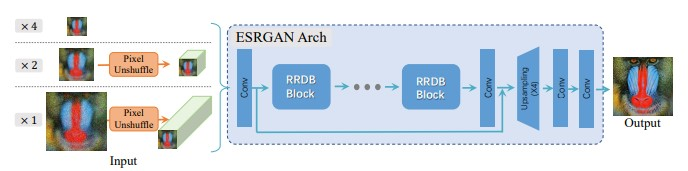
\includegraphics[height=2cm]{pic/pic0107.jpg}
        \caption{real-ESRGAN}
        \label{fig:0107}
    \end{figure}
    在ESRGAN基础上加了pixel-unshuffle模块.

    代码仓库环境配置较为容易, 成功训练, 结果很好.
\end{frame}

\begin{frame}{real-ESRGAN Result}
    
\end{frame}

\subsection{sinGAN}
\begin{frame}{sinGAN}{Single Natural Image GAN \href{https://github.com/tamarott/SinGAN}{GitHub Link}}
    sinGAN可用于但并非只可用于单张影像多尺度金字塔进行超分
    \begin{figure}
        \centering
        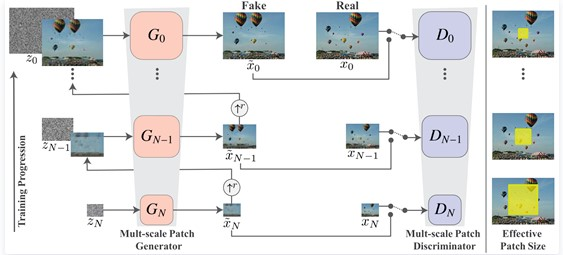
\includegraphics[height=4cm]{pic/pic0110.jpg}
        \caption{sinGAN}
        \label{fig:0110}
    \end{figure}
    
    优点: 只用一张影像非监督式(单张低分影像)

    缺点: 一次训练只能生成一张高分影像, 测试代码还在寻找
\end{frame}

\begin{frame}{sinGAN Result}
    \small
    \begin{figure}[!htbp]
        \centering
        \subfloat[input]{\label{fig:0111a}
        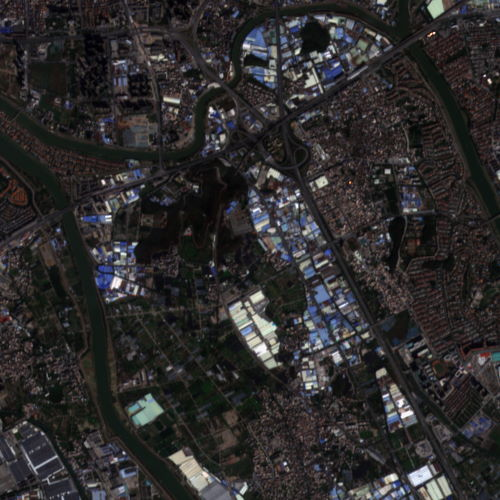
\includegraphics[height=5cm]{pic/pic0111a.jpg}}
        \quad
        \subfloat[output]{\label{fig:0111b}
        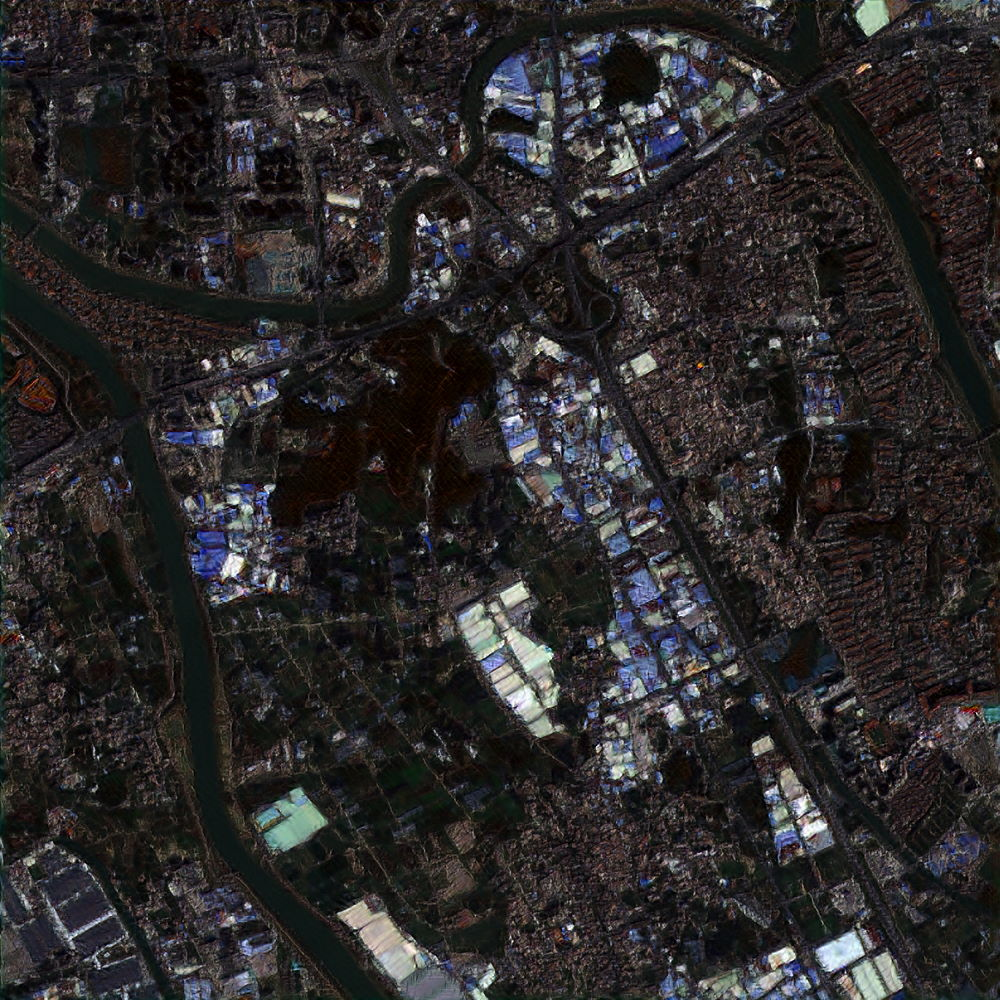
\includegraphics[height=5cm]{pic/pic0111b.jpg}}
        \caption{sinGAN}
        \label{fig:0111}
    \end{figure}
\end{frame}

% \begin{frame}{可用哨兵数据空间位置}
%     \small
%     考虑到六幅影像的范围有重叠, 只用其中一组即可
%     \begin{figure}
%         \centering
%         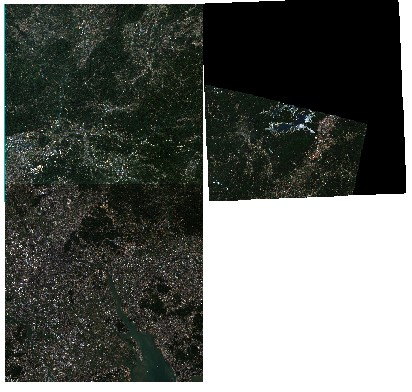
\includegraphics[width=6cm]{pic/pic0115.jpg}
%         \caption{哨兵可用重叠}
%         \label{fig:0109}
%     \end{figure}
% \end{frame}

% \begin{frame}{数据查询}
%     \begin{columns}
%         \column{0.3\textwidth}
%         \begin{itemize}
%             \item \small{对广东区域进行影像检索}
%         \end{itemize}

%         \column{0.7\textwidth}
%         \begin{figure}
%             \centering
%             % Requires \usepackage{graphicx}
%             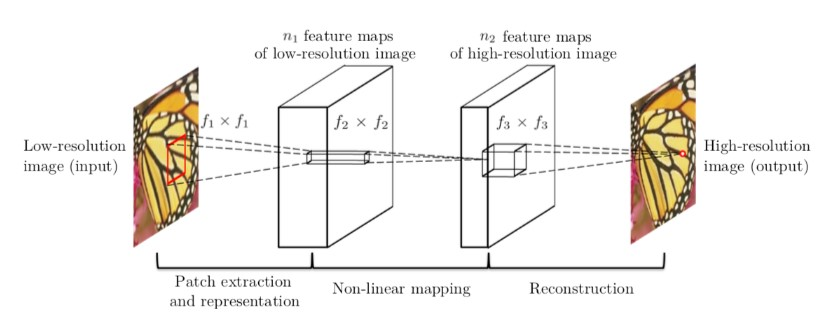
\includegraphics[width=5cm]{pic/pic0101.jpg}
%             \caption{影像查询地区}
%             \label{fig:0101}
%         \end{figure}
%     \end{columns}
% \end{frame}